\documentclass{article}

\usepackage{graphicx}
\usepackage{tikz}
\usepackage{tikzsymbols}
\usetikzlibrary{calc,patterns,shapes.geometric}
\pagestyle{empty}
\usepackage[margin=0pt]{geometry}
\geometry{papersize={14in,12in}}

\def\centerarc[#1](#2)(#3:#4:#5){\draw[#1] ($(#2)+({#5*cos(#3)},{#5*sin(#3)})$) arc (#3:#4:#5);}

\begin{document}
	\begin{figure}
		\centering
		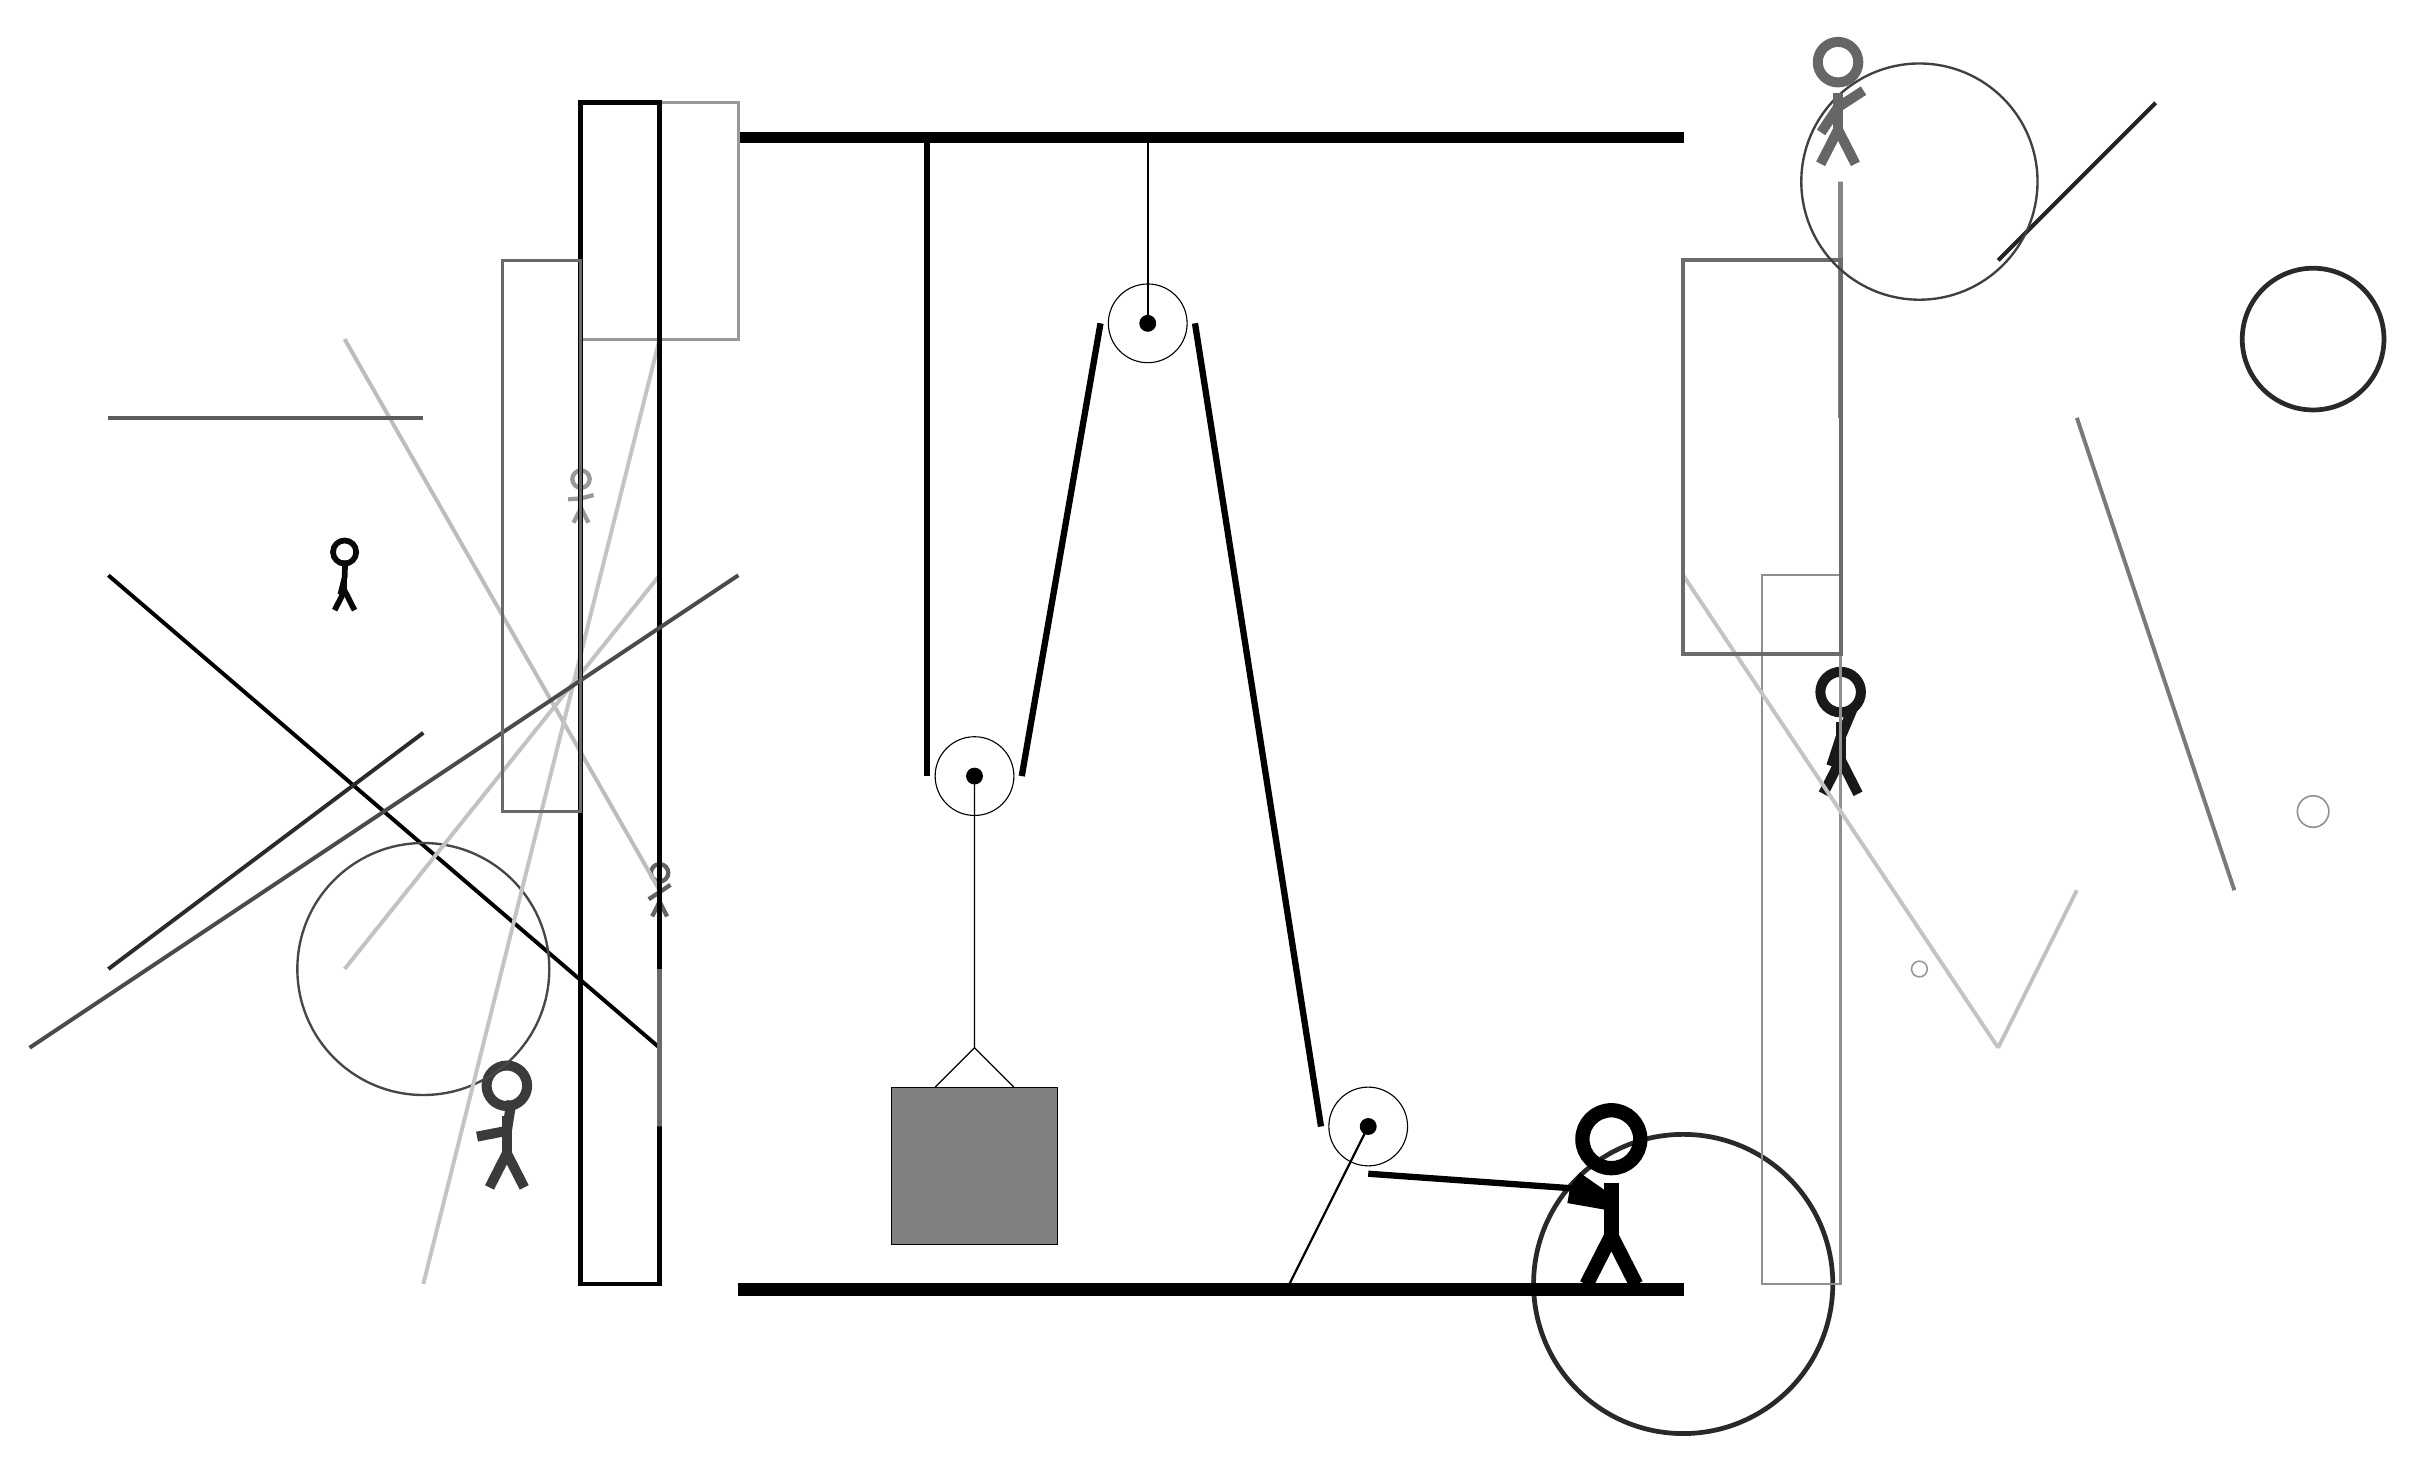
\begin{tikzpicture}
			%%%%% START %%%%%
			
			\draw[fill=black] (-2, 11.5) rectangle (10, 11.625);
			
			\draw[line width=0.5mm, color=black!24](15, 2) -- (14, 0);
			
			\draw[line width=0.5mm, color=black!100](-3, 0) -- (-10, 6);
			\node[line width=0.3mm, color=black!61] at (-3, 2) {\Strichmaxerl[3][33][34]};
			\draw [line width=0.6mm, color=black!84](10, -3) circle (1.9);
			\node[line width=0.3mm, color=black!40] at (-4, 7) {\Strichmaxerl[3][4][15]};
			\node[line width=0.2mm, color=black!77] at (-5, -1) {\Strichmaxerl[7][11][81]};
			\node[line width=0.3mm, color=black!90] at (12, 4) {\Strichmaxerl[7][72][67]};
			
			\draw[line width=0.5mm, color=black!26](-7, 9) -- (-3, 2);
			\draw [line width=0.2mm, color=black!41](13, 1) circle (0.1);
			\draw [line width=0.6mm, color=black!84](18, 9) circle (0.9);
			
			\draw[line width=0.6mm, color=black!48] (12, 11) rectangle (12, 8);
			\draw[line width=0.5mm, color=black!64](-6, 8) -- (-10, 8);
			\draw [line width=0.3mm, color=black!72](-6, 1) circle (1.6);
			
			\draw[line width=0.5mm, color=black!23](-3, 9) -- (-6, -3);
			\draw[line width=0.4mm, color=black!40] (-4, 12) rectangle (-2, 9);
			\draw[line width=0.3mm, color=black!44] (11, -3) rectangle (12, 6);
			
			\draw[line width=0.5mm, color=black!24](-3, 6) -- (-7, 1);
			\draw[line width=0.6mm, color=black!99] (-3, -3) rectangle (-4, 12);
			\draw[line width=0.7mm, color=black!59] (-3, -1) rectangle (-3, 1);
			\draw[line width=0.5mm, color=black!23](14, 0) -- (10, 6);
			\node[line width=0.7mm, color=black!97] at (-7, 6) {\Strichmaxerl[4][76][88]};
			
			\draw[line width=0.5mm, color=black!58] (10, 10) rectangle (12, 5);
			
			\draw[line width=0.5mm, color=black!86](14, 10) -- (16, 12);
			\draw[line width=0.5mm, color=black!71](-2, 6) -- (-11, 0);
			\draw[line width=0.4mm, color=black!59] (-4, 3) rectangle (-5, 10);
			
			\draw [line width=0.3mm, color=black!75](13, 11) circle (1.5);
			
			\draw [line width=0.2mm, color=black!44](18, 3) circle (0.2);
			\draw[line width=0.5mm, color=black!83](-6, 4) -- (-10, 1);
			\draw[line width=0.5mm, color=black!52](15, 8) -- (17, 2);
			\node[line width=0.7mm, color=black!60] at (12, 12) {\Strichmaxerl[7][56][33]};
			
			\draw (3.2, 9.2) circle (0.5);
			\draw[fill=black] (3.2, 9.2) circle (0.1);
			\draw[thick] (3.2, 9.2) -- (3.2, 11.5);
			
			\draw (6, -1) circle (0.5);
			\draw[fill=black] (6, -1) circle (0.1);
			\draw[thick] (6, -1) -- (5, -3);
			
			\draw (1, 3.45) circle (0.5);
			\draw[fill=black] (1, 3.45) circle (0.1);
			
			\draw (1, 3.45) -- (1, 0.0) -- (0.5, -0.5);
			\draw (1, 0.0) -- (1.5, -0.5);
			\draw[fill=black!50] (-0.05, -0.5) rectangle (2.05, -2.5);
			
			\draw[line width=0.8mm] (0.4, 11.5) -- (0.4, 3.45);
			\centerarc[line width=0.8mm](1, 3.45)(180:360:0.6);
			\draw[line width=0.8mm](1.6, 3.45) -- (2.6, 9.2);
			\centerarc[line width=0.8mm](3.2, 9.2)(0:180:0.6);
			\draw[line width=0.8mm](3.8, 9.2) -- (5.4, -1);
			\centerarc[line width=0.8mm](6, -1)(180:270:0.6);
			\draw[line width=0.8mm](6, -1.6) -- (8.8, -1.8);
			
			\node at (9, -1.9) {\Strichmaxerl[10][-35][170]};
			
			\draw[fill=black] (-2, -3) rectangle (10, -3.15);
			
			%%%%% END %%%%%
		\end{tikzpicture}
	\end{figure}	
\end{document}